\subsection*{Problem 8}
\iftoggle{contributions}{
\textit{Created by Tyler Wilson 2023}
}{}

A cylindrical capacitor has two concentric cylinders of radius $r_1$ and $r_2$ with length $L$. The inner cylinder is held at a charge $+Q$ and the outer cylinder is held at a charge $-Q$. Between these two cylinders is a liquid dielectric with dielectric constant $\kappa$ that comes up to a height $h$ with $h\leq L$.

\begin{center}
    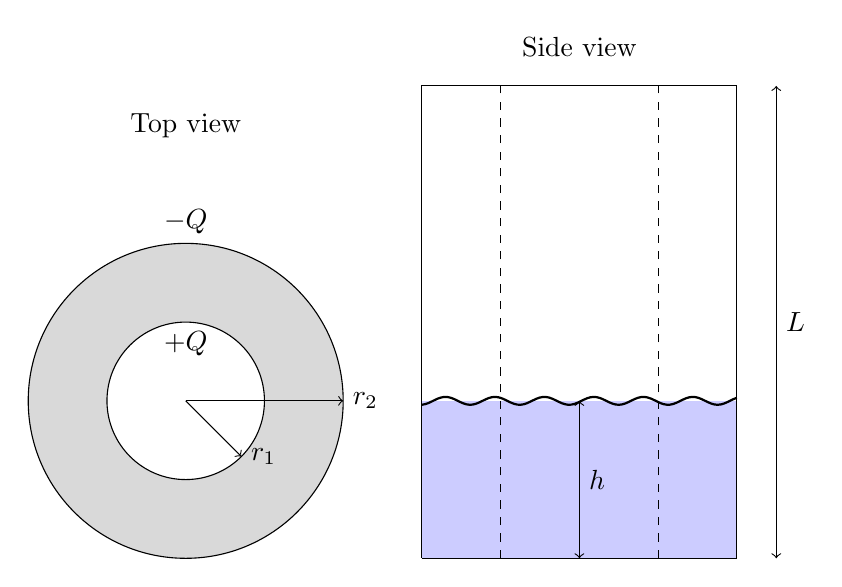
\begin{tikzpicture}
        \draw[fill=gray!30] (0,0) circle (2);
        \draw[fill=white] (0,0) circle (1);
        \draw[->] (0,0) -- (2,0) node[right] {$r_2$};
        \draw[->] (0,0) -- (0.707,-0.707) node[right] {$r_1$};
        \node[above] at (0,2) {$-Q$};
        \node[below] at (0,1) {$+Q$};
        \node at (0,3.5) {Top view};
        % side view
        \fill[blue!20] (3,-2) rectangle (7,0);
        \draw (3,-2) -- (3,4) -- (7,4) -- (7,-2) -- (3,-2);
        \draw[dashed] (4,-2) -- (4,4);
        \draw[dashed] (6,-2) -- (6,4);
        \draw[<->] (7.5,-2) -- (7.5,4);
        \node[right] at (7.5,1) {$L$};
        \draw[thick, domain=3:7, samples=100] plot (\x, {0.05*sin(10*\x r)});
        \draw[<->] (5,-2) -- (5,0);
        \node[right] at (5,-1) {$h$};
        \node at (5,4.5) {Side view};
    \end{tikzpicture}
\end{center}
\begin{enumerate}
    \item First let's assume that there is no dielectric between the two cylinders ($h=0$ case). In this case, find the capacitance of the cylinder in terms of the given variables ($r_1,\ r_2,\ L$).
    \item Now we will look at the case where $h\neq 0$. Find the capacitance of the cylinder in this case.\\
    \textit{Hint: It may be helpful to consider the system as two seperate capacitors being connected. You can use the result from part (a) to help you.}
    \item Find an expression for the energy in this capacitor.
    \item Compute the force acting on the dielectric due to the electric field.\\
    \textit{Hint: You can get the force from the energy by taking the negative gradient: $\vec{F}-\nabla U$. (In our case this will be $\vec{F}=\pdx[U]{h}\hat{j}$)}
    \item If the dielectric has a mass density of $\rho$, compute the equilibrium height of the dielectric.
\end{enumerate}

\iftoggle{solutions}{
\textbf{Solution:}
\begin{enumerate}
    \item The equation for capacitance is
    \[C=\frac{Q}{V}\]
    We have the charge $Q$ so we just need to find the potential difference $V$ between the two capacitor plates. We can find the potential difference by integrating the electric field from the inner cylinder to the outer cylinder.\\
    We can get the electric field between the plates using Gauss's law for a cylinder.
    \begin{align*}
        &\oiint\vec{E}\cdot d\vec{A}=\frac{q_\text{enc}}{\epsilon_0}\\
        &q_\text{enc}=Q\\
        &EA=\frac{Q}{\epsilon_0}\\
        &E=\frac{Q}{\epsilon_0A}=\frac{Q}{\epsilon_0(2\pi rL)}=\frac{Q}{2\pi\epsilon_0 rL}
    \end{align*}
    We can then integrate the electric field from the inner cylinder to the outer cylinder to get the potential difference.
    \begin{align*}
        &\Delta V=-\int_{r_2}^{r_1}E dr\\
        &\Delta V=-\int_{r_2}^{r_1}\frac{Q}{2\pi\epsilon_0 rL} dr\\
        &\Delta V=-\frac{Q}{2\pi\epsilon_0 L}\int_{r_2}^{r_1}\frac{dr}{r}\\
        &\Delta V=-\frac{Q}{2\pi\epsilon_0 L}\ln(r)\eval_{r_2}^{r_1}\\
        &\Delta V=-\frac{Q}{2\pi\epsilon_0 L}\ln\left(\frac{r_1}{r_2}\right)\\
        &\Delta V=\frac{Q}{2\pi\epsilon_0 L}\ln\left(\frac{r_2}{r_1}\right)
    \end{align*}
    Now we can find the capacitance.
    \begin{align*}
        &C=\frac{Q}{\Delta V}\\
        &C=\frac{Q}{\frac{Q}{2\pi\epsilon_0 L}\ln\left(\frac{r_2}{r_1}\right)}\\
        &\answer{C=\frac{2\pi\epsilon_0 L}{\ln\left(\frac{r_2}{r_1}\right)}}
    \end{align*}
    \item We can analyse this problem by considering the system as two seperate capacitors. The first capacitor is the same as the one from part (a) but with length $L-h$. The second capacitor is the one formed by the dielectric and will be of length $h$. These two capacitors are connected side by side so we can imagine that they are connected in parallel and so the total capacitance can be gotten by adding the two capacitors in parallel.
    \begin{align*}
        &C_1=\frac{2\pi\epsilon_0 (L-h)}{\ln\left(\frac{r_2}{r_1}\right)}\\
        &C_2=\frac{2\pi\epsilon_0 h\kappa}{\ln\left(\frac{r_2}{r_1}\right)}\\
        &C_\text{total}=C_1+C_2\\
        &C_\text{total}=\frac{2\pi\epsilon_0 (L-h)}{\ln\left(\frac{r_2}{r_1}\right)}+\frac{2\pi\epsilon_0 h\kappa}{\ln\left(\frac{r_2}{r_1}\right)}\\
        &\answer{C_\text{total}=\frac{2\pi\epsilon_0}{\ln\left(\frac{r_2}{r_1}\right)}(L+h(\kappa-1))}\\
    \end{align*}
    \item The energy in a capacitor is given by
    \[U=\frac{1}{2}CV^2\]
    We can rearrange this equation to get it in terms of $C$ and $Q$
    \begin{align*}
        &C=\frac{Q}{V}\Ra V=\frac{Q}{C}\\
        &U=\frac{1}{2}CV^2=\frac{1}{2}C\left(\frac{Q}{C}\right)^2=\frac{1}{2}CQ^2
    \end{align*}
    We can then plug in the values we computed earlier to get the energy.
    \begin{align*}
        &U=\frac{1}{2}CQ^2\\
        &U=\frac{1}{2}\left(\frac{2\pi\epsilon_0}{\ln\left(\frac{r_2}{r_1}\right)}(L+h(\kappa-1))\right)Q^2\\
        &\answer{U=\frac{\pi\epsilon_0Q^2}{\ln\left(\frac{r_2}{r_1}\right)}(L+h(\kappa-1))}
    \end{align*}
    \item The force can be computed using the derivative of the potential energy with respect to the height.
    \begin{align*}
        &\vec{F}=\pdx[U]{h}\hat{j}\\
        &\vec{F}=\pdx{h}\left(\frac{\pi\epsilon_0Q^2}{\ln\left(\frac{r_2}{r_1}\right)}(L+h(\kappa-1))\right)\hat{j}\\
        &\answer{\vec{F}=\frac{\pi\epsilon_0Q^2}{\ln\left(\frac{r_2}{r_1}\right)}(\kappa-1)\hat{j}}
    \end{align*}
    \item At equilibrium the net force on the dielectric will be zero. There is a force from the electric field pulling the dielectric up into the cylinder and the opposing force of gravity pulling it downward. We can set these two forces equal to each other and solve for the height.
    \begin{align*}
        &F_g=F_E\\
        &F_E=\frac{\pi\epsilon_0Q^2}{\ln\left(\frac{r_2}{r_1}\right)}(\kappa-1)\\
        &F_g=mg\\
        &\rho=\frac{m}{V}\Ra m=\rho V\\
        &F_g=\rho Vg\\
        &V=\pi (r_2^2-r_1^2)h\\
        &F_g=\rho\pi (r_2^2-r_1^2)hg\\
        &\frac{\pi\epsilon_0Q^2}{\ln\left(\frac{r_2}{r_1}\right)}(\kappa-1)=\rho\pi (r_2^2-r_1^2)hg\\
        &h=\frac{\frac{\pi\epsilon_0Q^2}{\ln\left(\frac{r_2}{r_1}\right)}(\kappa-1)}{\rho\pi (r_2^2-r_1^2)g}\\
        &\answer{h=\frac{\epsilon_0Q^2(\kappa-1)}{\rho\ln\left(\frac{r_2}{r_1}\right)(r_2^2-r_1^2)g}}
    \end{align*}
\end{enumerate}
}{}
